\documentclass{jarticle}

\usepackage[dvipdfmx]{graphicx}
\usepackage{url}
\usepackage{listings,jlisting}
\usepackage{ascmac}
\usepackage{amsmath,amssymb}

%ここからソースコードの表示に関する設定
\lstset{
    basicstyle={\ttfamily},
    identifierstyle={\small},
    commentstyle={\smallitshape},
    keywordstyle={\small\bfseries},
    ndkeywordstyle={\small},
    stringstyle={\small\ttfamily},
    frame={tb},
    breaklines=true,
    columns=[l]{fullflexible},
    numbers=left,
    xrightmargin=0zw,
    xleftmargin=3zw,
    numberstyle={\scriptsize},
    stepnumber=1,
    numbersep=1zw,
    lineskip=-0.5ex
}
%ここまでソースコードの表示に関する設定 

\title{知能プログラミング演習II 課題4}
\author{グループ07\\
    29114007 池口 弘尚\\
    29114031 大原 拓人\\
    29114048 北原 太一\\
    29114086 飛世 裕貴\\
    29114095 野竹 浩二朗\\
%  {\small (グループレポートの場合は、グループ名および全員の学生番号と氏名が必要)}
}
\date{2019年11月26日}

\begin{document}
\maketitle

\paragraph{提出物} このレポート グループプログラム"group07.zip"
\paragraph{グループ} グループ07
\paragraph{グループ} グループ07
\paragraph{メンバー}
\begin{tabular}{|c|c|c|}
    \hline
    学生番号&氏名&担当箇所\\
    \hline\hline
    29114007&池口弘尚&4-3,4-4\\
    \hline
    29114031&大原拓人&4-3\\
    \hline
    29114048&北原太一&4-1\\
    \hline
    29114086&飛世裕貴&4-2\\
    \hline
    29114095&野竹浩二朗&4-2,4-4\\
    \hline
\end{tabular}

\section{課題の説明}
\begin{description}
    \item[必須課題4-1] まず,教科書3.2.1の「前向き推論」のプログラムと教科書3.2.2の
    「後向き推論」のプログラムとの動作確認をし,前向き推論と後ろ向き推論の違いを説明せよ.
    また,実行例を示してルールが選択される過程を説明せよ.説明の際には,LibreOfficeの
    Draw(コマンド soffice --draw)などのドロー系ツールを使ってp.106 図3.11や
    p.118 図3.12のような図として示すことが望ましい.
    \item[必須課題4-2] CarShop.data , AnimalWorld.data 等のデータファイルを
    実際的な応用事例(自分達の興味分野で良い)に書き換えて,前向き推論,
    および後ろ向き推論に基づく質問応答システムを作成せよ.どのような応用事例を扱うかは,メンバーで話し合って決めること.
    なお,ユーザの質問は英語や日本語のような自然言語が望ましいが,難しければ変数を含むパターン等でも可とする.
    \item[必須課題4-3] 上記4-2で実装した質問応答システムのGUIを作成せよ.
    質問に答える際の推論過程を可視化できることが望ましい.
    \item[発展課題4-4] 上記4-3で実装したGUIを発展させ,質問応答だけでなく,
    ルールの編集(追加,削除,変更)などについてもGUIで行えるようにせよ.
\end{description}
\section{課題4-1}
\begin{screen}
    まず,教科書3.2.1の「前向き推論」のプログラムと教科書3.2.2の
    「後向き推論」のプログラムとの動作確認をし,前向き推論と後ろ向き推論の違いを説明せよ.
    また,実行例を示してルールが選択される過程を説明せよ.説明の際には,LibreOfficeの
    Draw(コマンド soffice --draw)などのドロー系ツールを使ってp.106 図3.11や
    p.118 図3.12のような図として示すことが望ましい.
\end{screen}
\subsection{実行例29114048-北原太一}
\subsubsection{前向き推論}
まず、デフォルトのまま前向き推論のRuleBaseSystem.javaを
実行した時における推論過程を図\ref{fig:FCCS}に示す。
なお、一番上の点線で囲まれたアサーションは元々ワーキングメモリ上
にあることを表す。

 \begin{figure}[htbp]
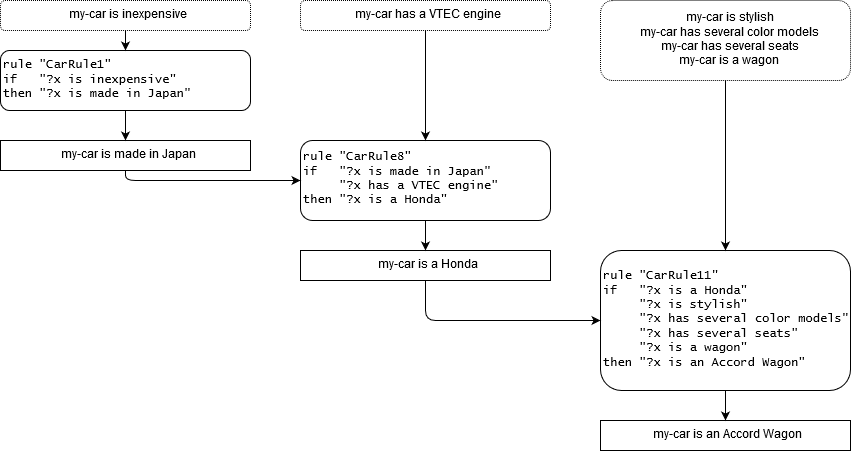
\includegraphics[scale=0.35]{048/Forward1.png}
\caption{前向き推論:CarShop.data}
\label{fig:FCCS}
\end{figure}

次に、AnimalWorld.dataを利用するためにRuleBaseSystem.java
のRuleBaseクラスのコンストラクタの一部をソースコード
\ref{lst:FCAW}のように変えた。

  \begin{lstlisting}[caption=RuleBase2.java(一部抜粋),label=lst:FCAW]
fileName = "AnimalWorld.data";
wm = new WorkingMemory();
wm.addAssertion("my-friend has hair");
wm.addAssertion("my-friend eats meat");
wm.addAssertion("my-friend has tawny color");
wm.addAssertion("my-friend has black");
  \end{lstlisting}
  
このプログラムを実行した時における推論過程を
図\ref{fig:FCAW}に示す。
 
\begin{figure}[htbp]
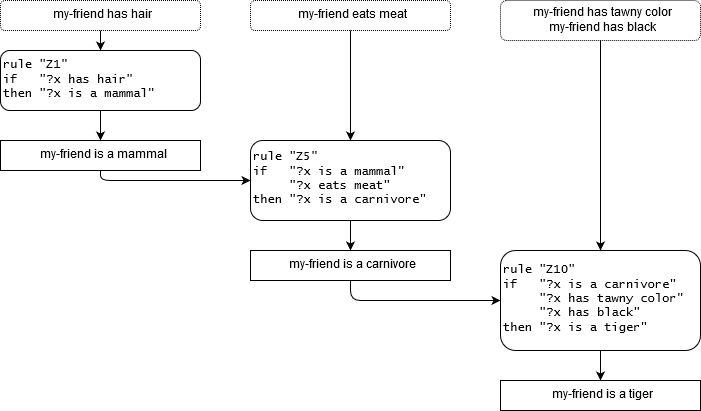
\includegraphics[scale=0.35]{048/Forward2.png}
\caption{前向き推論:AnimalWorld.data}
\label{fig:FCAW}
\end{figure}


\subsubsection{後向き推論}

まず、デフォルトのまま後向き推論のRuleBaseSystem.javaを
ソースコード\ref{lst:BCCS}に示すコマンドで実行した。

\begin{lstlisting}[caption=後ろ向き推論1,label=lst:BCCS]
>java RuleBaseSystem "?x is an Accord Wagon"
\end{lstlisting}

この実行における推論過程を図\ref{fig:BCCS}に示す。なお、矢印の隣の括弧つき数字はルールの適用順を、(WM)はワーキングメモリ上のアサーションを、矢印上の×印はワーキングメモリ上のアサーションと一致しなかったことを表す。

\begin{figure}[htbp]
%jarticleでこの通りにすると小さすぎて読めません
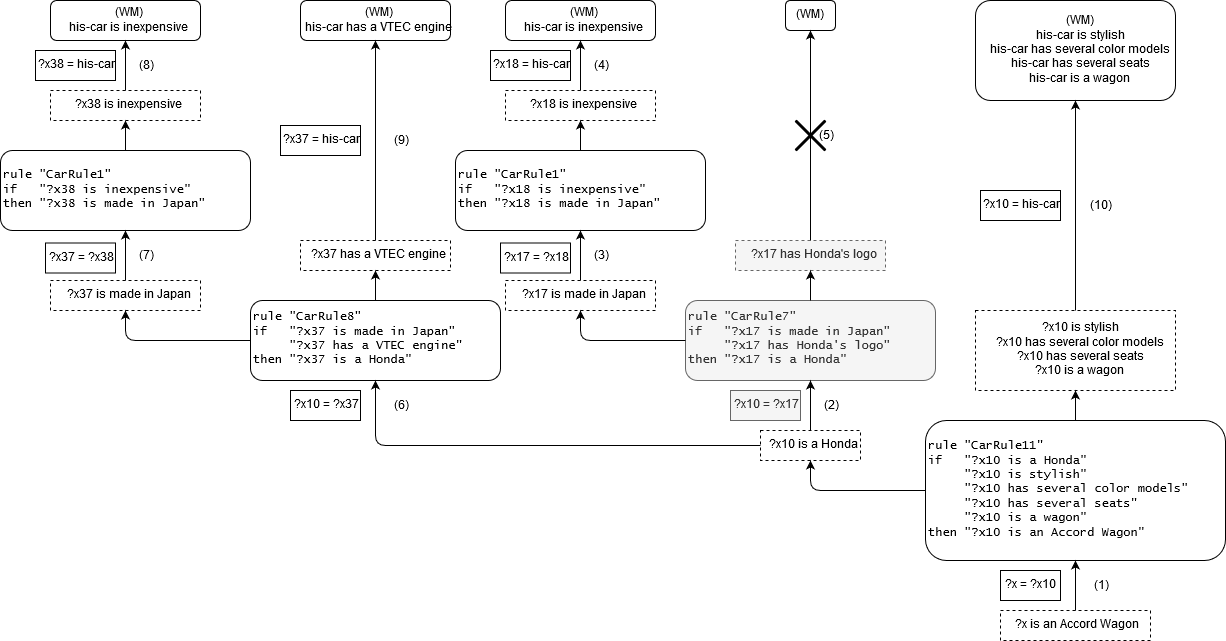
\includegraphics[scale=0.25]{048/Backward1.png}
\caption{後向き推論:CarShop}
\label{fig:BCCS}
\end{figure}


次に、デフォルトのRuleBaseSystem.javaのコメントアウトを付け替え、
CarShop.data, CarShopWm.dataの代わりにAnimalWorld.data, 
AnimalWorldWm.dataを使用するようにしたうえでソースコード
\ref{lst:BCAW}に示すコマンドを実行した。

\begin{lstlisting}[caption=後向き推論2,label=lst:BCAW]
>java RuleBaseSystem "?x is giraffe"
\end{lstlisting}

この実行における推論過程をCarShopの場合と同じように
図\ref{fig:BCAW}に示す。

\begin{figure}[htbp]
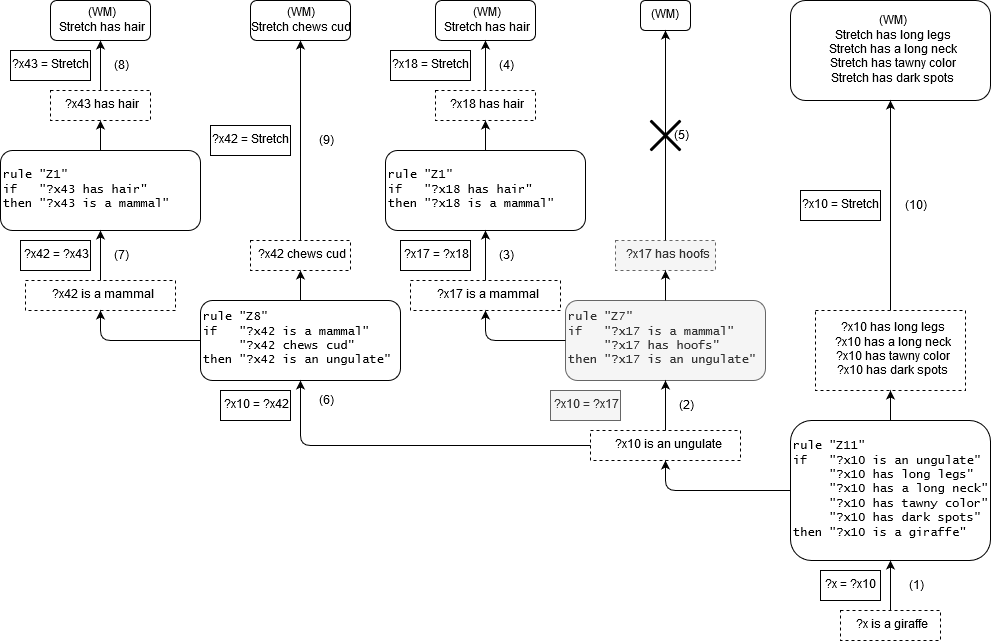
\includegraphics[scale=0.30]{048/Backward2.png}
\caption{後向き推論:AnimalWorld}
\label{fig:BCAW}
\end{figure}


\subsection{考察29114048-北原太一}

前向き推論では、すでにワーキングメモリ上にあるアサーションからルールを適用して新しいアサーションを導く。すなわち、すでにある知識から新しい知識を導く手法といえる。また、後向き推論では、与えられたパターンにルールを適用し、新しいパターンを作り、最後にワーキングメモリ上のパターンとマッチングさせる。すなわち、仮定にどの知識が合致する、あるいは当てはまるかを導く手法といえる。\\
 この両者の大きな違いとして、ワーキングメモリの使い方を挙げることができる。すなわち、前向き推論においてはワーキングメモリが推論のスタート地点であり、後向き推論においてはワーキングメモリが推論のゴール地点である。

\section{課題4-2}
\begin{screen}
    CarShop.data , AnimalWorld.data 等のデータファイルを
    実際的な応用事例(自分達の興味分野で良い)に書き換えて,前向き推論,
    および後ろ向き推論に基づく質問応答システムを作成せよ.どのような応用事例を扱うかは,メンバーで話し合って決めること.
    なお,ユーザの質問は英語や日本語のような自然言語が望ましいが,難しければ変数を含むパターン等でも可とする.
\end{screen}
\subsection{手法29114031-大原拓人}
私は自然言語(英語)によって質問を解釈する質問応答システムを担当した。
時間内に完成できなかったため、考察のみ記す。

\subsection{考察29114031大原拓人}
自然言語で質問を解釈するシステムを作成するにあたって、解決すべき課題は
以下のようになった。
\begin{enumerate}
\item 疑問詞を検出し変数に置き換える
\item 疑問詞の種類によって変数を配置する場所が異なる
\item 文脈によって変数を配置する場所が異なる
\item クエリと異なり、答えとなる部分は1語ではない
\item 3人称になったときの動詞の活用、名詞の複数形を検出する
\end{enumerate}
以上に挙げたものの解決策を挙げていくと、
\begin{enumerate}
\item OpenNLPのライブラリを用いて、文節chunkに分けることで
    「whose car」のようなかたまりを検出できるので、それを変数に置き換えればよい
\item 疑問詞の種類自体は少ないので、switch文で場合分けをすればよい
\item これといった解決策が思いつかなかった。パターン照合のシステムと
    連携して複数のパターンを探索する形であれば実現の可能性がある。
\item こちらも、パターン照合のシステムに変数が1つ、2つ、3つ...のそれぞれの
    パターンを引数として渡すことで実現の可能性がある。
\item OpenNLPのライブラリに、用いられている単語が3人称の動詞や
    複数形であっても、原型が何であるかを返すメソッドがあるので
    パターン照合のシステム上に組み込むことで、比較が可能になる。
\end{enumerate}
しかし、以上に挙げた解決策を実装すると、文脈検出の探索と、複数単語の回答のための探索で
プログラムの命令数が爆発的に増えると予想される。つまり、ルールや照合すべきパターンが増えると
実用的な時間内に結果を返すことができない恐れがある。
この爆発的な増加を抑える方法を模索していたが、時間内に
その方法を見つけ出すことができなかったので実装には至らなかった。
\subsection{手法29114086-飛世裕貴}
本課題ではスポーツに関するデータファイルを作成し、そのデータファイルを用いて前向き推論、後ろ向き推論に基づく質問応答システムを作成する.以下に今回用いるデータファイル(data.txt、dataWm.txt)の一部を示す.\\

\begin{screen}
\begin{verbatim}

rule 	"Rule1"
if 	"We play ?x indoors"
then 	"?x is an indoor sport"

rule 	"Rule2"
if 	"We play ?x outdoors"
then 	"?x is an outdoor sport"

rule 	"Rule3"
if 	"We use a ball in ?x"
then 	"?x is a ball sport"

rule 	"Rule4"
if 	"?x is a ball sport"
	"We use a racket in ?x"
then 	"?x is a racket sport"

rule 	"Rule5"
if 	"?x is an indoor sport"
	"?x is a ball sport"
	"We play ?x in 5 people"
then 	"?x is basketball"
\end{verbatim}
\vdots
(後略)

\end{screen}
\begin{center}
図1:ルールベースに関するデータファイル(data.txt)の一部\\
\end{center}


\begin{screen}
\begin{verbatim}

my-club-activity is an indoor sport
We use a ball in my-club-activity
my-club-activity is a sport over the net
We play my-club-activity in 6 people
His-competition is swimming
We runs 800 meter to 5000 meter on his-competition

\end{verbatim}
\end{screen}
\begin{center}
図2:ワーキングメモリに関するデータファイル(dataWm.txt)\\
\end{center}
このようなデータファイルを用いて、質問応答システムを作成していく.尚、質問応答システムの作成に関してはパターンマッチングによる質問応答機能を作成したあと、自然言語に対応させていくという流れで進行していく.私は後ろ向き推論におけるパターンマッチングによる質問応答機能の作成を担当した.

\subsection{実装29114086-飛世裕貴}
パターンマッチングにおいてルールベース、ワーキングメモリの読み込みをloadRules、loadWmメソッドで行い、後ろ向き推論による質問応答は既存のRuleBaseクラスのbackwardChainメソッドを用いて行った.ここでワーキングメモリを読み込む際、図2に示したように数字をトークンとして読み込むと正しく読み込まれず、質問応答が正しく行われない.そのため、loadWmメソッドを以下のように実装した.\\

\begin{lstlisting}[caption=loadWmメソッド]
  public ArrayList<String> loadWm(String theFileName){
    ArrayList<String> wm = new ArrayList<String>();
    String line;
    try{
      int token;
      f = new FileReader(theFileName);
      st = new StreamTokenizer(f);
      st.eolIsSignificant(true);
      st.wordChars('\'','\'');
      while((token = st.nextToken())!= StreamTokenizer.TT_EOF){
        line = new String();
        while( token != StreamTokenizer.TT_EOL){
          //以下、変更点
          if(st.sval == null)
            line = line + (int)st.nval + " ";
          else
            line = line + st.sval + " ";
          token = st.nextToken();
        }
        wm.add(line.trim());
      }
    } catch(Exception e){
      LogArea.println(e);
    }
    return wm;
  }

\end{lstlisting}

\begin{verbatim}

\end{verbatim}
変更を加えたのは上記プログラム中の14〜17行目で、読み込んだトークンが文字列でなければ数値として扱うようにしている.
このようにする事でワーキングメモリ中の「We play my-club-activity in 6 people」のようにトークンとして数字を含む場合においても質問応答が可能となった.

\subsection{実行例29114086-飛世裕貴}
後ろ向き推論に関するプログラムを実行したとき、その結果を標準出力に出力したものを以下に示す.\\

\begin{screen}
\begin{verbatim}
Enter data-filename:data.txt
Enter workingmemory-filename:dataWm.txt
add rule? delete rule? add...1/delete...2/No thanks...3 :3
Enter Search pattern:?x is volleyball
Hypothesis:[?x is volleyball]
Success RULE
Rule:Rule6 [?x5 is an indoor sport, ?x5 is a ball sport, 
?x5 is a sport over the net,We play ?x5 in 6 people]
->?x5 is volleyball <=> ?x is volleyball
\end{verbatim}
\vdots
(中略)\\
\vdots
\begin{verbatim}
Success WM
We play my-club-activity in 6 people <=> We play ?x5 in 6 people
Yes
{?x=my-club-activity, ?x5=my-club-activity, ?x8=my-club-activity}
binding: {?x=my-club-activity, ?x5=my-club-activity, ?x8=my-club-activity}
tmp: ?x, result:  my-club-activity
Query: ?x is volleyball
Answer:my-club-activity is volleyball
\end{verbatim}
\end{screen}
\begin{center}
図3:後ろ向き推論による質問検索の実行例\\
\end{center}

このようにトークンとして数字を含んでいたとしても正しく検索ができていることを確認できた.
\subsection{考察29114086-飛世裕貴}
今回の課題ではトークンとして数字が含まれている場合においても
検索できるように改良を加えたが、「5000 meter」を「5000m」
のように略記した際には単一トークン中に数字と文字が含まれること
でトークン読み込みが正しく行われず、検索も正常に行われない事
がわかった.このような問題は自然言語における形態素解析によっ
て解決できるのではないかと考えられる.トークンという考え方に
おいては「5000m」のような文字列は一つのトークンとして認識
してしまうために正常に検索が行えなかったが、この文字列を
形態素解析器に読み込ませると「5000」と「m」という二つの
形態素として認識する事ができる.そのため、一つのトークンを
文字列部と数字部に分離して考える事ができる.一例として、実際
に文字と数字を含む文字列に対して形態素解析器MeCabを用いて
形態素解析を行なった結果を以下に示しておく.\\

\begin{screen}
\begin{verbatim}
5000m
5000	名詞,数,*,*,*,*,*
m	名詞,固有名詞,組織,*,*,*,*
EOS

G7サミット
G	名詞,一般,*,*,*,*,*
7	名詞,数,*,*,*,*,*
サミット	名詞,一般,*,*,*,*,サミット,サミット,サミット
EOS
\end{verbatim}
\end{screen}
\begin{center}
図4:形態素解析による文字と数字の分割の実行例
\end{center}
このようにトークンとしてではなくさらに細かい分割である
形態素を用いることで、より一般的な文字列に対して正常な検索
が可能な質問検索システムを実装する事が可能であると考える.

\subsection{手法29114095-野竹浩二朗}
この課題ではスポーツに関するデータファイルを作成し,そのデータを用いて前向き推論、後ろ向き推論に基づいて処理をしていく。
私は自然言語ではなく、パターンによる処理ができるプログラムを作成した。

\subsection{実装29114095-野竹浩二朗}
データファイルの中身は以下のようになっている。
\begin{screen}
\begin{verbatim}
rule "Rule1"
if "We play ?x in the water"
then "?x is swimming"

rule "Rule2"
if "?x is swimming"
   "?x can be any way of swimming"
then "?x is freestyle"

rule "Rule3"
if "?x is swimming"
   "?x strokes hands in front of chest"
   "?x move one kick backward"
then "?x is breaststroke"
\end{verbatim}
\end{screen}
パターン認識には、以前の課題で作成したUnifyクラスを用いて、今回のRuleBaseSystem.javaのメインメソッドに以下のコードを追加した。
\begin{lstlisting}[caption=追加したコード]
    while(true){
      System.out.print("Enter Search Pattern:");
      String query = stdIn.nextLine();
      if(query.equals("exit")){
        break;
      }
      for(String st:rb.wm.assertions){
        (new Unifier()).unify(st,query);
      }
    }
\end{lstlisting}
「Enter Search Pattern:」の後に「We play ?x indoors」のように入力することで、入力されたパターンとマッチする文を出力する。

また、データファイル名、ワーキングメモリを書き込んだファイル名を読み込めるよう、RuleBaseクラスのRuleBaseメソッドに以下を追加した。
\begin{lstlisting}[caption=RuleBaseメソッド]
    System.out.print("Enter data-filename:"); // ファイル名の入力
    fileName = scan.nextLine();
    wm = new WorkingMemory();
    fm = new FileManager();

    System.out.print("Enter workingmemory-filename:");
    dataFilename = scan.nextLine();
    ArrayList<String> wms = fm.loadWm(dataFilename); //ワーキングメモリの取り込み
    for(String str : wms){
      wm.addAssertion(str);
    }
\end{lstlisting}
ルールやワーキングメモリに入れる文を変更する場合は、データファイルを変更する。

\subsection{実行例29114095-野竹浩二朗}
DataBaseSystemを実行した結果を以下に示す。ルールを追加する際、Rule1からRule34までが羅列されてしまい、実行結果が長くなってしまうため、一部省略している。(「...」の部分)
\begin{lstlisting}
Enter data-filename:data.txt
Enter workingmemory-filename:dataWm.txt
ADD:We play tennis outdoors
ADD:We use a ball in tennis
ADD:We use racket in tennis
Rule1 [We play ?x indoors]->?x is an indoor sport
Rule2 [We play ?x outdoors]->?x is an outdoor sport
...(中略)
Rule33 [?x is throwing competitions, We throw a hammmer in ?x]->?x is hammer throw
Rule34 [?x is throwing competitions, We throw a spear]->?x is javelin
apply rule:Rule1
apply rule:Rule2
Success: tennis is an outdoor sport
ADD:tennis is an outdoor sport
apply rule:Rule3
Success: tennis is a ball sport
ADD:tennis is a ball sport
apply rule:Rule4
apply rule:Rule5
...(中略)
apply rule:Rule33
apply rule:Rule34
Working Memory[We play tennis outdoors, We use a ball in tennis, We use racket in tennis, tennis is an outdoor sport, tennis is a ball sport]
No rule produces a new assertion

Enter Search Pattern:We play ?x indoors
Enter Search Pattern:We play ?x ?y
{?x=tennis, ?y=outdoors}
Enter Search Pattern:exit
\end{lstlisting}
ルールとワーキングメモリを読み込んだ後、探索するパターンを入力した結果を見ると、dataWm.txtの中身のデータとマッチする要素を取り出せていることが分かる。
\subsection{考察29114095-野竹浩二朗}
私が作成したプログラムでは、入力されたパターンによる検索しかできない。入力された文を単語ごとに分け、キーとなる単語、今回ではplayやindoorなどを識別することができれば自然言語処理に近い形ができると考えられる。
このプログラムでは、データファイルに「800m」といった数字と文字が混ざった単語の処理がうまくできず、ユーザーが使える文法が制限されてしまっている。数字が入っていても単に文字列として読み込むことができれば改善すると考えられる。

\section{課題4-3}
\begin{screen}
    上記4-2で実装した質問応答システムのGUIを作成せよ.
    質問に答える際の推論過程を可視化できることが望ましい.
\end{screen}
\subsection{手法29114007-池口弘尚}
課題4-2で作成した探索をカプセル化し、GUI側からそれを呼び出すことによって実装した。

\subsection{実装29114007-池口弘尚}
基本的な構造は今までと同じなので省略する。
今回で新たに使用したのは、JTextFieldでエンターを押したときの判定の取り方である。

\begin{lstlisting}[caption=JTextFieldのActionListener,label=src:text]
public ForwardSearchPanel(String name, kadai4.ForwardChain.RuleBaseSystem rbs) {
	(略)
	ActionListener searchActionListener = new ActionListener() {
		@Override
		public void actionPerformed(ActionEvent e) {
			rbs.patternSearch(text1.getText());
			text1.setText("");
		}
	};
	text1.addActionListener(searchActionListener);
	button.addActionListener(searchActionListener);
}
\end{lstlisting}
上のコードのように今までボタンに付けていたActionListenerをJTextFieldにも加えることによって、入力のわずらわしさを減らすことができた。

また、今回はそれぞれのパネルをJTabbedPaneを使用してタブで分けた。
そのために今まで使ってきたFrameBaseを継承してPageFrameBaseを以下のように作成した。
\begin{lstlisting}[caption=PageFrameBase,label=src:PageFrameBase]
public class PageFrameBase extends FrameBase {
	JTabbedPane tabbedpane;

	public PageFrameBase(String title, int x, int y, int width, int height, PagePanelBase[] pages) {
		super(title, x, y, width, height);
		MakePages(pages);
	}

	public PageFrameBase(String title, int width, int height, PagePanelBase[] pages) {
		super(title, width, height);
		MakePages(pages);
	}
	//ページを作成
	private void MakePages(PagePanelBase[] pages) {
		JPanel p = new JPanel();

		tabbedpane = new JTabbedPane();
		for (PagePanelBase Panel : pages) {
			tabbedpane.add(Panel, Panel.getName());
		}
		//tabbedpane.setSize(1600, 100);

		LogArea logArea = new LogArea(30, 140);
		SpringLayout layout = new SpringLayout();
		p.setLayout(layout);

		layout.putConstraint(SpringLayout.NORTH, tabbedpane, 5, SpringLayout.NORTH, p);
		layout.putConstraint(SpringLayout.SOUTH, tabbedpane, 305, SpringLayout.NORTH, p);
		layout.putConstraint(SpringLayout.EAST, tabbedpane, -30, SpringLayout.EAST, p);
		layout.putConstraint(SpringLayout.WEST, tabbedpane, 30, SpringLayout.WEST, p);

		layout.putConstraint(SpringLayout.NORTH, logArea, 10, SpringLayout.SOUTH, tabbedpane);
		layout.putConstraint(SpringLayout.HORIZONTAL_CENTER, logArea, 0, SpringLayout.HORIZONTAL_CENTER, p);

		p.add(tabbedpane);
		p.add(logArea);
		add(p, BorderLayout.CENTER);
	}

}
\end{lstlisting}
PagePanelBaseはJPanelに名前を持たせただけのクラスなので説明は省く。

課題2の時にはそれぞれのログは別で表示されていたが、今回はPageFrameBaseでログエリアを作成することによって共通で使えるようにしてある。
また、今回の課題では過程を表示しなければならないため、どこからでもログを表示できる必要があった。
そのため、LogAreaは以下のように実装した。

\begin{lstlisting}[caption=Log,label=src:log]
public class LogArea extends JScrollPane {
	static LogArea instance;
	JTextArea area;
	JViewport viewport;

	public LogArea(int rows, int columns) {
		super();
		area = new JTextArea(rows, columns);
		EtchedBorder border = new EtchedBorder(EtchedBorder.RAISED);
		area.setEditable(false);
		area.setBorder(border);
		setViewportView(area);
		viewport = getViewport();
		instance = this;
	}
	//1行ログを表示
	public static void println(String txt) {
    	//インスタンスが無ければSystem.out
		if (instance != null)
			instance.area.append(txt + "\n");
		else
			System.out.println(txt);
	}
	//続けてログを表示
	public static void print(String txt) {
    	//インスタンスが無ければSystem.out
		if (instance != null)
			instance.area.append(txt);
		else
			System.out.print(txt);
	}
}
\end{lstlisting}
これは、GUIが作成されていなければSystem.outが使われるため、作業段階から利用することができる。

\subsection{実行例29114007-池口弘尚}
\begin{figure}[!hbt]
  \centering
  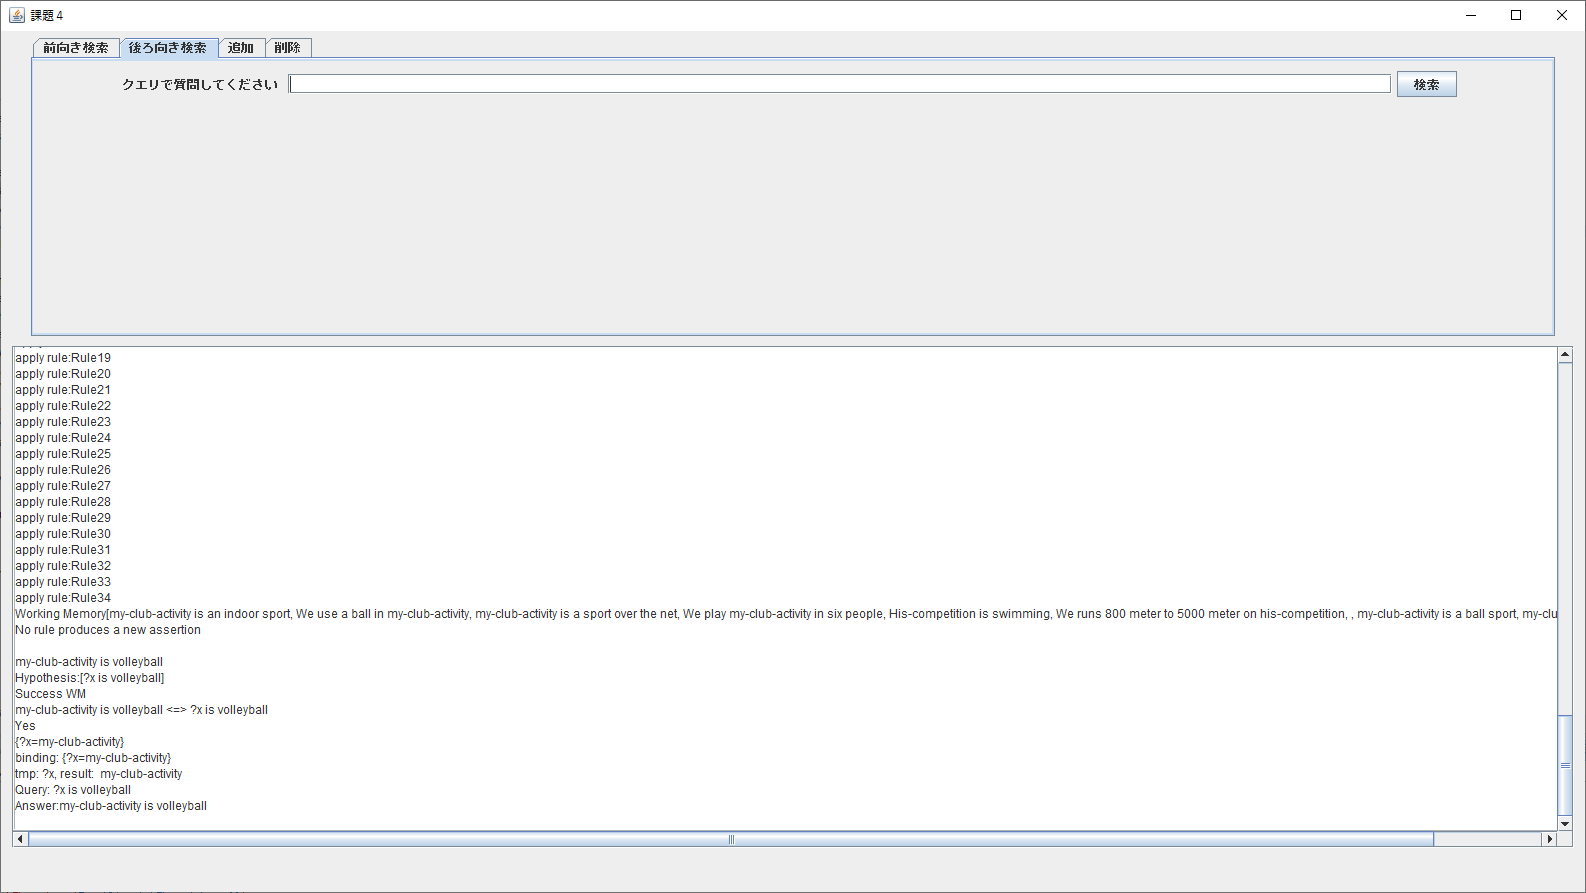
\includegraphics[scale=0.25]{007/GUI1.png}
  \caption{検索例}
  \label{fig:Search}
\end{figure}
\subsection{考察29114007-池口弘尚}
外側のメソッドを呼ぶだけなので問題は生じなかった。

\section{課題4-4}
\begin{screen}
    上記4-3で実装したGUIを発展させ,質問応答だけでなく,
    ルールの編集(追加,削除,変更)などについてもGUIで行えるようにせよ.
\end{screen}
\subsection{手法29114007-池口弘尚}
今までと同様な手法によってGUIに追加する。
変更に関しては、削除してから新たに追加することとした。
\subsection{実装29114007-池口弘尚}
GUI部分に関しては今までと変わらないため説明は省く。
RuleBase部分を編集してルールの追加などを行えるようにした。
\begin{lstlisting}[caption=編集,label=src:Change]
//ルールを1つ追加
public void addRules(String name, ArrayList<String> antecedents, String consequent) {
	rules.add(new Rule(name, antecedents, consequent));
}
//ルール名で削除
public void deleteRules(String name) {
	for (int i = 0; i < rules.size(); i++) {
		if (rules.get(i).getName().equals(name)) {
			LogArea.println("Delete:" + rules.get(i));
			rules.remove(i);
			i--;
		}
	}
}
//アサーションを削除
public void deleteAssertion(String assertion) {
	wm.assertions.remove(assertion);
}
//ルールをまとめて追加
public void addRules(List<Rule> rules) {
	for (Rule rule : rules) {
		if (!this.rules.contains(rule)) {
			LogArea.println("Add:" + rule);
			this.rules.add(rule);
		}
	}
}
//アサーションをまとめて追加
public void addWorkingMemory(List<String> wmlist) {
	for (String string : wmlist) {
		wm.addAssertion(string);
	}
}
//アサーションを1つ追加
public void addWorkingMemory(String wmline) {
	wm.addAssertion(wmline);
}
\end{lstlisting}

\newpage
\subsection{実行例29114007-池口弘尚}
\begin{figure}[!hbt]
  \centering
  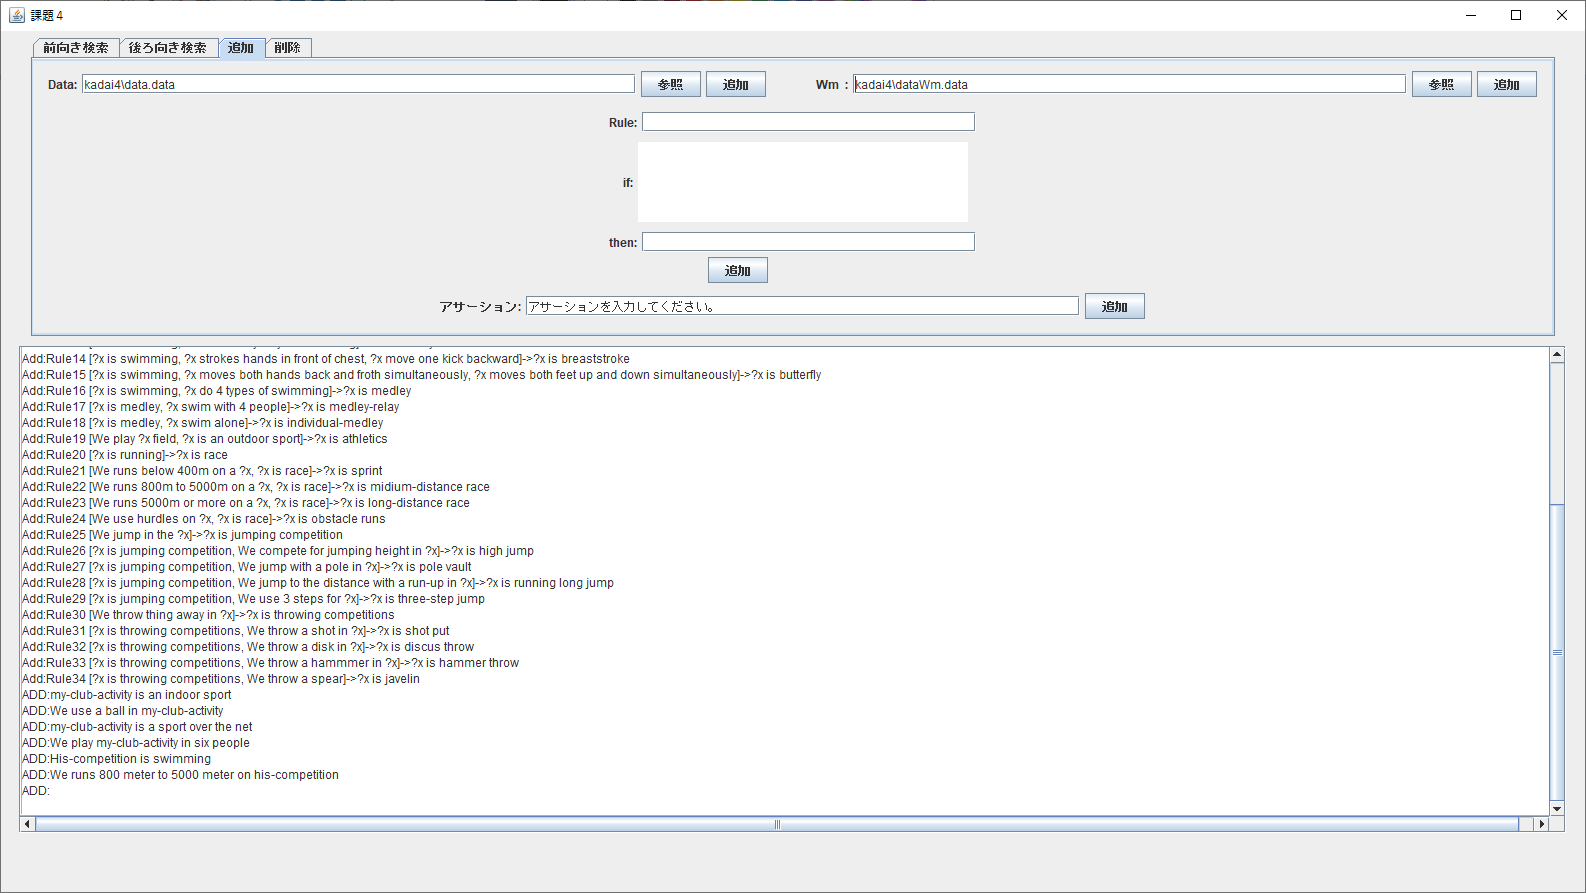
\includegraphics[scale=0.25]{007/GUI2.png}
  \caption{追加例}
  \label{fig:Add}
  \centering
  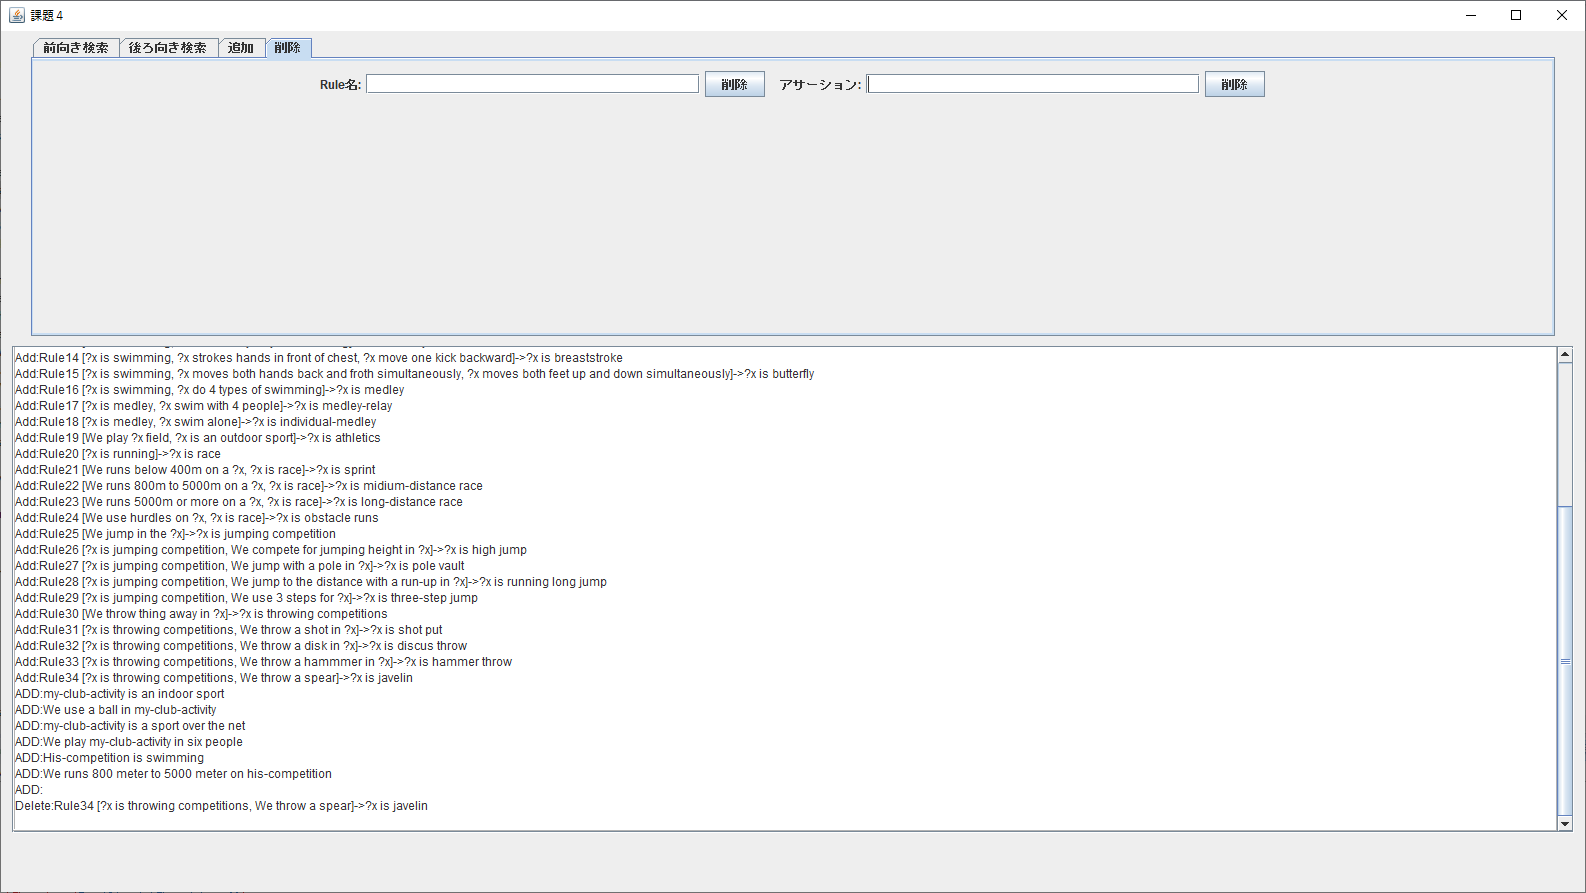
\includegraphics[scale=0.25]{007/GUI3.png}
  \caption{削除例}
  \label{fig:Remove}

  
\end{figure}
\subsection{考察29114007-池口弘尚}
追加や削除を行うときにそれが存在しているかなどの判定が甘いため、想定している通りの操作以外のことをすると上手く動かない可能性がある。
\subsection{手法29114095-野竹浩二朗}
ルールを追加・削除するメソッドを作成し、それを用いてGUIからルールの追加、削除を行えるようにする。
\subsection{実装29114095-野竹浩二朗}
私は、ルールを追加できるメソッド\\
addRulesと削除できるメソッドdeleteRulesを作成した。
まず、addRulesを示す。
\begin{lstlisting}[caption=addRulesメソッド]
void addRules(String name,ArrayList<String> antecedents,String consequent){
rules.add(new Rule(name,antecedents,consequent));
}
}
\end{lstlisting}
ルール名、条件、結果を引数とし、その要素をまとめてルールを格納しているArrayListであるrulesに格納する。
次に、ルールを削除するdeleteRulesを示す。
\begin{lstlisting}[caption=deleteRulesメソッド]
void deleteRules(String name){
  for(int i=0; i<rules.size();i++){
    if(rules.get(i).getName().equals(name)){
      rules.remove(i);
      i--;
    }
  }
}
}
\end{lstlisting}
ルールを削除する際はルール名のみを引数とする。rules.get(i).getName()により、ルール名を順に呼び出し、入力されたルール名と一致したとき、rules.remove()により、要素を削除する。

ルールを追加する際、既存のルール名と被ってはいけないため、新たに入力されたルール名と既存のルール名を比較するjudgeNameメソッドも追加した。以下にその中身を示す
\begin{lstlisting}[caption=judgenameメソッド]
boolean judgeName(String name){
  boolean judge = true;
  while(true){
    for(int i=0; i<rules.size();i++){
      if(rules.get(i).getName().equals(name)){
        judge = true;
        break;
      }else{
        judge = false;
        break;
      }
    }
    break;
  }
  return judge;
}
\end{lstlisting}
このメソッドでは、入力されたルール名と既存のルール名が被っていた場合にtrueを返すようになっている。
また、メインメソッドには、ルールの追加、削除、何もしないと選べるよう、switch文を用いて分岐を加えた。
\begin{lstlisting}[caption=メインメソッドに追加した文]
    System.out.print("add rule? delete rule? add...1/delete...2/No thanks...3 : ");
    int j = stdIn.nextInt();

    switch(j){
      case 1:
		...
      case 2:
      	...
      case 3:
      	...
    }
\end{lstlisting}
switch文の中身をすべて記述すると無駄に長くなってしまうため省略した。
case 1では入力されたルール名と既存のルール名を比較したのちにルールを追加する。
case 2ではルール名を入力し、ルールを削除するようになっている。
case 3では何もせずに次の操作に移る。

\subsection{実行例29114095-野竹浩二朗}
ルールの追加、削除するメソッドを追加したDataBaseSystemを実行した結果を以下に示す。
\begin{lstlisting}
Enter data-filename:data.txt
Enter workingmemory-filename:dataWm.txt
...(中略)
Rule33 [?x is throwing competitions, We throw a hammmer in ?x]->?x is hammer throw
Rule34 [?x is throwing competitions, We throw a spear]->?x is javelin
add rule? delete rule? add...1/delete...2/No thanks...3 :1
--- Add Rule !!! ---
Enter RuleName:Rule35
Enter antecedent:We play ?x space
finish
Enter consequent:?x is unknown
...(中略)
apply rule:Rule34
apply rule:Rule35
Working Memory[We play tennis outdoors, We use a ball in tennis, We use racket in tennis, tennis is an outdoor sport, tennis is a ball sport]
No rule produces a new assertion
...(以下略)
\end{lstlisting}
ここでも、実行結果を省略して載せている。ルールの追加を選択後、3つの要素を入力するとaplly ruleにルールが反映されていることが確認できる。
\subsection{考察29114095-野竹浩二朗}
ルールを削除する際、ルール名を把握しなければならない。今回ではRuleXXというルールの番号が分かっていないと削除できないため、ルールの内容から検索、削除ができるようになればさらに汎用性が高いものができると考えたが、効率的にルールを検索する方法が思いつかず、今回はルール名を指定して削除する方法となってしまった。

\section{感想29114007-池口弘尚}
コードの設計をどのようにするのかなどを取り決めていなかったため、
中途半端な実装になってしまった。
例えば、RuleBaseがForwardとBackwardで分かれていたために
同じような機能が別のもので実装されていたり、MatcherとUnifierが
存在したりするといったことである。
そのため、次回からは作ったクラスやメソッドを
リストアップしていく必要があると思った。
\section{感想29114031-大原拓人}
今回実装が間に合わなかった要因として、自然言語での質疑応答システムが予想以上に複雑であったことと、
完全な自然言語への対応を妥協し、もう少し単純なシステムで解決しようとしなかったことが挙げられる。
グループのメンバーと相談し、ある程度の妥協案を出しておくべきであった。
\section{感想29114095-野竹浩二朗}
今回の課題では、BackwordChain、ForwordChainの2つがあり、
片方でできてももう片方ではできなかったりと苦労した。
また、GUIを作ったわけではないが、GUIを作るうえで使う
メソッドを作成した。これに関してGUIの作成を担当してくれている人
からどんなメソッドの方がいいかを聞きながらの作成となったので大変だった。

% 参考文献
\begin{thebibliography}{99}
    \bibitem{pl} ウェブインテリジェンスの演習で用いられたコードの例を参考にした
    \bibitem{is} 新谷虎松,講義「知識システム」スライド
\end{thebibliography}

\end{document}